\documentclass{hipatia}
\usepackage{lipsum}
%Use \DeclareMathOperator para definir novos
% operadores para o modo matemático
\DeclareMathOperator{\sen}{sen}

%Evite numerar teoremas
%Prefira nomeá-los
%Use os ambientes abaixo
\newtheorem*{theorem*}{Teorema}
\newtheorem*{lemma*}{Lema}
\newtheorem*{corollary*}{Corolário} % Para criar o ambiente de definição não numerado
\theoremstyle{definition} % Altera o estilo para texto normal
\newtheorem*{definition*}{Definição} % Para criar o ambiente de definição não numerado

\newcommand{\superau}{\textsuperscript{\underline{a}}~}

% Evite títulos muito longos
%\title{Acaso e Certezas: A Versatilidade \\do Método Probabilístico}
% Se for necessário diminuir a fonte do título 
% para caber no quadro, use
 \title{ \fontsize{28}{28}\selectfont Caminhando por Sequências de Farey}

% O Subtítulo é o nome da seção da revista
% Deve ser uma palavra de origem grega
\subtitle{Técnica}
\author{Carlos Augusto D. Ribeiro}
% A data não é necessária
%\date{October 2023}
% Não se preocupe com a numeração
% das páginas ou com o número da edição

\begin{document}

\maketitle

\section{Introdução}

Este artigo foi inspirado pelo Problema 6 da Olimpíada Brasileira de Matemática (OBM) e da Olimpíada Brasileira de Matemática Universitária (OBMU) de 2024. Durante a pesquisa por materiais de referência em português sobre as sequências de Farey, tornou-se evidente a escassez de artigos ou publicações que tratassem do tema de forma acessível e aprofundada. A maioria do conhecimento disponível está restrita a artigos e livros em inglês, limitando o acesso a estudantes e entusiastas da matemática sem fluência nesse idioma.

Com isso, este artigo pretende preencher essa lacuna, reunindo resultados e conceitos de diversas fontes em inglês e organizando-os de forma clara e didática. O objetivo principal é fornecer um material útil tanto para matemáticos amadores curiosos quanto para estudantes avançados envolvidos em olimpíadas de matemática. As sequências de Farey são um tópico rico em propriedades e padrões interessantes, com aplicações que transcendem a teoria dos números, alcançando áreas como geometria e aproximação de números irracionais. Espero que este material inspire o interesse e expanda o horizonte matemático de todos os que explorarem estas páginas.

\section{A História Peculiar das Sequências de Farey}
A história das sequências de Farey é marcada por uma curiosa reviravolta, envolvendo um geólogo, um matemático renomado e um matemático menos conhecido. A sequência leva o nome de John Farey, um geólogo inglês que, em 1816, publicou um artigo intitulado ``On a curious property of vulgar fractions'' na revista Philosophical Magazine. Neste artigo, Farey observou um padrão interessante nas frações entre 0 e 1, organizadas em ordem crescente e com denominadores limitados por um determinado valor. Ele descreveu como construir a sequência, listou os termos da sequência de ordem 5 como exemplo e questionou se a propriedade já havia sido observada ou demonstrada anteriormente.

Um dos leitores do artigo de Farey foi ninguém menos que Augustin-Louis Cauchy, um dos matemáticos mais proeminentes da época. Cauchy, impressionado pela observação de Farey, forneceu uma demonstração rigorosa da propriedade no mesmo ano. A partir de então, a sequência passou a ser conhecida como ``sequência de Farey'', consolidando o nome de Farey na história da matemática.

A ironia, porém, é que Farey não foi o primeiro a descobrir as propriedades da sequência. Charles Haros, um matemático menos conhecido, já havia, em 1802, identificado a propriedade e até mesmo explicado como construir a 99\superau sequência. Infelizmente para Haros, seu trabalho não recebeu o reconhecimento devido na época, e ele acabou sendo ofuscado pela publicação de Farey.

O caso das sequências de Farey ilustra como a história da matemática, assim como outras áreas do conhecimento, pode ser permeada por acasos e injustiças. Farey, apesar de sua contribuição modesta, acabou imortalizado por uma descoberta que não era originalmente sua. Em \textit{A Mathematician's Apology}, G. H. Hardy comenta ironicamente: ``... Farey é imortal porque não conseguiu entender um teorema que Haros havia provado perfeitamente quatorze anos antes...''.

Apesar da controvérsia em torno da autoria das descobertas sobre suas propriedades, as sequências de Farey passaram a ser estudadas na teoria dos números, com diversas aplicações, incluindo a aproximação racional de números irracionais e contribuições importantes à geometria. 



\section{Construção das Sequências de Farey}

Em todos os resultados, demonstrações e soluções daqui em diante, assumiremos que as frações estão em sua forma irredutível, salvo indicação em contrário. Existem diversas formas de introduzirmos as sequências de Farey, desde uma definição pragmática até a construção de diagramas onde os andares nos dão a respectiva sequência de ordem $n$.

Para fins didáticos, iniciemos com o algoritmo para a construção, que nos levará a um diagrama, e por fim chegaremos à definição limpa e direta. Começamos com a sequência de ordem 1, representada por:
\[
F_1 = \left\{ \frac{0}{1}, \frac{1}{1} \right\}.
\]

Para construir a sequência de ordem \(n\), denotada por \(F_n\), a partir da sequência de ordem \(n-1\), denotada por \(F_{n-1}\), siga os seguintes passos de forma detalhada:

\begin{enumerate}
    \item \textbf{Inicialize a nova sequência:} 
    \begin{itemize}
        \item Comece copiando todos os elementos da sequência \(F_{n-1}\) para uma nova sequência, que chamaremos de \(F_n\). Assim, a nova sequência \(F_n\) inicialmente é uma cópia de \(F_{n-1}\).
    \end{itemize}

    \item \textbf{Calcule e insira as mediantes:} 
    \begin{itemize}
        \item Para cada par de frações consecutivas \(\frac{a}{b}\) e \(\frac{a'}{b'}\) em \(F_{n-1}\), calcule a fração mediante entre elas, dada pela fórmula:
        \[
        \text{Mediante} = \frac{a + a'}{b + b'}
        \]
        \item A fração mediante é obtida somando os numeradores e os denominadores das frações consecutivas.
    \end{itemize}

    \item \textbf{Verifique a condição do denominador:}
    \begin{itemize}
        \item Após calcular a fração mediante \(\frac{a + a'}{b + b'}\), verifique se o denominador resultante, \(b + b'\), é menor ou igual a \(n\). Isto é importante, pois queremos limitar o tamanho do denominador para garantir que a sequência \(F_n\) respeite a ordem definida.
        \item Se a condição \(b + b' \leq n\) for satisfeita, então a fração mediante deve ser inserida entre \(\frac{a}{b}\) e \(\frac{a'}{b'}\) na sequência \(F_n\).
        \item Caso contrário, se \(b + b' > n\), a fração mediante não é adicionada, e seguimos para o próximo par de frações consecutivas em \(F_{n-1}\).
    \end{itemize}
    
    \item \textbf{Concluindo a construção da sequência:}
    \begin{itemize}
        \item Repita o processo para todos os pares consecutivos de frações em \(F_{n-1}\). Ao final, a sequência \(F_n\) estará completa, contendo tanto as frações da sequência anterior quanto as novas frações mediantes que foram inseridas, respeitando o limite do denominador.
    \end{itemize}
\end{enumerate}



De forma geral, esse processo pode ser resumido no diagrama a seguir:

\begin{figure}[h]
    \centering
    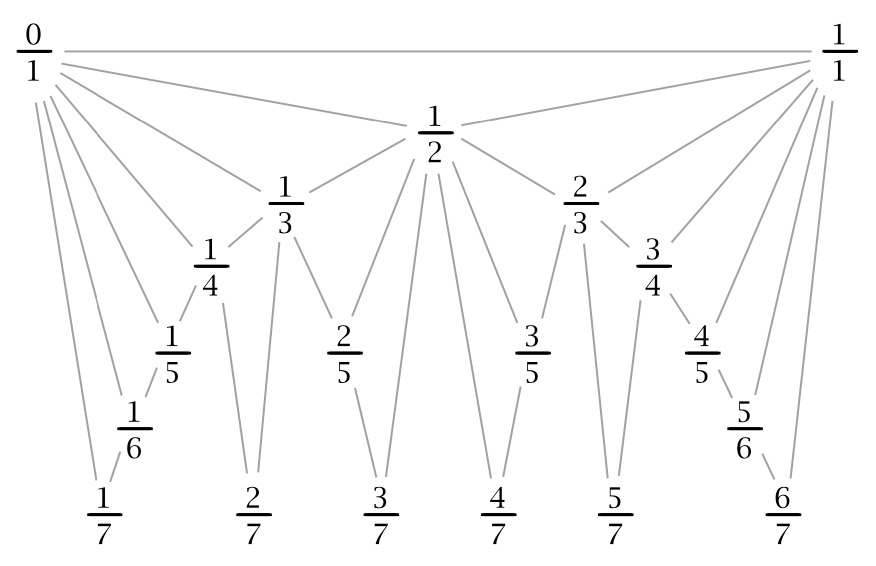
\includegraphics[width=1\linewidth]{diagrama.jpeg}
    %\caption{Enter Caption}

\end{figure}



Finalmente, uma definição direta da sequência de Farey de ordem \( n \):

\begin{definition*}
    A \textit{sequência de Farey de ordem \( n \)}, denotada por \( F_n \), é o conjunto de frações racionais \(\frac{r}{s}\), onde \(0 \leq r \leq s \leq n\), com \(\text{mdc}(r, s) = 1\), dispostas em ordem crescente, incluindo os extremos \(0 = \frac{0}{1}\) e \(1 = \frac{n}{n}\). 
\end{definition*}
    Cabe observar que cada elemento da sequência de Farey é uma fração irredutível cujo denominador é menor ou igual a \(n\). Além disso, a sequência \(F_n\) contém todas as frações que podem ser formadas nesse intervalo, de modo que frações consecutivas satisfazem a condição de estarem na menor forma e ordenadas de maneira crescente.


\section{Propriedades básicas}

Nesta seção, começamos explorando a relação fundamental entre frações consecutivas, descrita pelo Teorema da Vizinhança de Farey (TVF). Este teorema nos fornece uma condição necessária e suficiente para que duas frações sejam vizinhas em uma sequência de Farey de ordem n. Tal critério é extremamente útil, pois permite identificar quais frações são mais próximas em termos de aproximação racional e também serve como base para outros resultados.

\begin{theorem*} (da Vizinhança de Farey)
As frações \(\frac{a}{b} < \frac{c}{d}\) são consecutivas na sequência de Farey \(F_n\) se, e somente se, \(bc - ad = 1\) e $b+d\geq n+1$.
\end{theorem*}

\begin{proof}
Como \(\operatorname{mdc}(a, b) = 1\), a equação linear \(bx - ay = 1\) tem uma solução \(x = x_0\), \(y = y_0\). Além disso, \(x = x_0 + at\), \(y = y_0 + bt\) também será uma solução para qualquer inteiro \(t\). Escolha \(t = t_0\) de forma que
\begin{align*}
0 \leq n - b < y_0 + bt_0 \leq n
\end{align*}
e defina \(x = x_0 + bt_0\), \(y = y_0 + bt_0\). Como \(y \leq n\), \(\frac{x}{y}\) será uma fração em \(F_n\). Além disso,
\[
\frac{x}{y} = \frac{a}{b} + \frac{1}{by} > \frac{a}{b}
\]
de modo que \(\frac{x}{y}\) aparece depois na sequência de Farey do que \(\frac{a}{b}\). Se \(\frac{x}{y} \neq \frac{c}{d}\), então \(\frac{x}{y} > \frac{c}{d}\) e obtemos
\begin{align*}
\frac{x}{y} - \frac{c}{d} = \frac{dx - cy}{dy} \geq \frac{1}{dy}
\end{align*}
bem como
\begin{align*}
\frac{c}{d} - \frac{a}{b} = \frac{bc - ad}{bd} \geq \frac{1}{bd}.
\end{align*}
Somando as duas desigualdades, obtemos
\begin{align*}
\frac{x}{y} - \frac{a}{b} \geq \frac{1}{dy} + \frac{1}{bd} = \frac{b + y}{bdy}.
\end{align*}
Mas \(b + y > n\) (lembre que \(n - b < y\)) e \(d \leq n\), resultando na contradição
\begin{align*}
\frac{1}{by} = \frac{bx - ay}{by} = \frac{x}{y} - \frac{a}{b} = \frac{b + y}{bdy} > \frac{n}{bdy} \geq \frac{1}{by}.
\end{align*}
Assim, \(\frac{x}{y} = \frac{c}{d}\) e a equação \(bx - ay = 1\) torna-se \(bc - ad = 1\).
\end{proof}

Daqui em diante, sempre que nos referirmos a frações que são termos consecutivos de uma sequência de Farey, usaremos o termo \textit{vizinhas de Farey} para nos referirmos às mesmas. 

O corolário a seguir, que nomearemos de Corolário da Mediante, revela uma característica interessante sobre frações consecutivas: a fração intermediária entre duas vizinhas de Farey é obtida através da soma dos numeradores e denominadores, resultando na chamada fração mediante. Esse corolário reforça a ideia de simetria e estrutura nas sequências de Farey, mostrando que frações mediantes surgem naturalmente e estão posicionadas entre as frações originais, conforme esperado.

\begin{corollary*} (da Mediante)
Se $\frac{a}{b}<\frac{a'}{b'}<\frac{a''}{b''}$ são vizinhas de Farey contidas em \(F_n\), então
\[
\frac{a'}{b'}=\frac{a+a''}{b+b''}.
\]

\end{corollary*}

\begin{proof} Aplicando o TVF aos pares adjacentes:

1) Para \(\dfrac{a}{b}\) e \(\dfrac{a'}{b'}\):

\[
b'a - ba' = 1. \quad (1)
\]

2) Para \(\dfrac{a'}{b'}\) e \(\dfrac{a''}{b''}\):

\[
b''a' - b'a'' = 1. \quad (2)
\]

Subtraindo a equação (1) da equação (2):

\[
(b''a' - b'a'') - (b'a - ba') = 1 - 1,
\]

\[
(b''a' - b'a'') - (b'a - ba') = 0.
\]

Simplificando:

\[
b''a' - b'a'' - b'a + ba' = 0,
\]

\[
a'(b'' + b) - b'(a'' + a) = 0.
\]

Reorganizando:

\[
a'(b + b'') = b'(a + a'').
\]

Assim, obtemos:

\[
\dfrac{a'}{b'} = \dfrac{a + a''}{b + b''}.
\]


\end{proof}

Vale notar que uma das consequências importantes do Teorema das Frações Vizinhas (TVF) foi estabelecer uma cota mínima para a soma dos denominadores de duas frações vizinhas, cota essa que se verifica ser a melhor possível. Uma pergunta natural que emerge é: será que para três frações vizinhas também existe uma cota mínima para a soma de seus denominadores? A resposta é afirmativa. Por ora, apresentaremos uma cota mínima menos refinada, reservando para a seção de Problemas Olímpicos a demonstração da melhor cota possível (que apareceu como problema 6 na OBM de 2024!).

\begin{corollary*} (da Cota Mínima)
Se $\frac{a}{b}<\frac{a'}{b'}<\frac{a''}{b''}$ são frações vizinhas de Farey contidas em \(F_n\), então
\[
b+b'+b''\geq \left\lceil \frac{4(n+1)}{3} \right\rceil.
\]
\end{corollary*}

\begin{proof}
    Do corolário anterior, sabemos que $\dfrac{a'}{b'} = \dfrac{a + a''}{b + b''}$. Seja então $d=(a+a'',b+b'')$. Logo o TVF nos dá que:
    $$
    b+\frac{b+b''}{d}\geq n+1\quad \text{ e } \quad b''+\frac{b+b''}{d}\geq n+1,
    $$
\noindent donde obtemos que 
$$
\begin{aligned}
\left(b+\frac{b+b^{\prime \prime}}{d}\right)+\left(b^{\prime \prime}+\frac{b+b^{\prime \prime}}{d}\right) & \geqslant 2(n+1) \\
\Rightarrow \quad b+b^{\prime \prime} & \geqslant \frac{2 d(n+1)}{d+2}.
\end{aligned}
$$
Assim, vale que 
$$
\begin{aligned}
b+b^{\prime}+b^{\prime \prime} & =b+b^{\prime \prime}+\frac{b+b^{\prime \prime}}{d} \\
& =\left(b+b^{\prime \prime}\right) \frac{(d+1)}{d} \\
& \geqslant \frac{2 d}{d+2} \cdot(n+1) \frac{(d+1)}{d} \\
& =2(n+1) \frac{(d+1)}{d+2}\\
&\geq 2(n+1) \frac{2}{3}.
\end{aligned}
$$

Segue o resultado.
    
\end{proof}


Como próximo resultado, temos o que chamaremos de Corolário da Aproximação, pois ele quantifica a diferença entre uma fração e sua mediante. Essa estimativa não apenas caracteriza a aproximação entre frações, mas também demonstra como as mediantes são eficientes em dividir o espaço racional de maneira equilibrada. Este resultado, além de sua importância teórica, possui implicações práticas em problemas de aproximação racional de números reais.

\begin{corollary*}[da Aproximação]
Se \(\frac{a}{b}\) e \(\frac{a'}{b'}\) são vizinhas de Farey contidas em \(F_n\), então
\[
\left| \frac{a}{b} - \frac{a + a'}{b + b'} \right| = \frac{1}{b(b + b')} \leq \frac{1}{b(n + 1)},
\]
e
\[
\left| \frac{a'}{b'} - \frac{a + a'}{b + b'} \right| = \frac{1}{b'(b + b')} \leq \frac{1}{b'(n + 1)}.
\]
\end{corollary*}



\begin{proof}
Usando o \textit{TVF}, sabemos que:
\begin{align*}
\left| \frac{a}{b} - \frac{a + a'}{b + b'} \right| &= \frac{|a(b + b') - b(a + a')|}{b(b + b')} \\
&= \frac{|ab + ab' - ab - ba'|}{b(b + b')} = \frac{1}{b(b + b')}.
\end{align*}
Então, como sabemos que \(b + b' \geq n + 1\), podemos substituir
\[
\left| \frac{a}{b} - \frac{a + a'}{b + b'} \right| = \frac{1}{b(b + b')} \leq \frac{1}{b(n + 1)}.
\]

Basta repetir esses passos para provar que a segunda desigualdade também é verdadeira.
\end{proof}

O resultado a seguir mostra que, se tomarmos frações vizinhas em uma metade da sequência, há uma correspondência direta com frações na outra metade, formando um espelho perfeito. Essa propriedade é fundamental para compreender a estrutura palíndroma das sequências de Farey, uma característica que será explorada mais a fundo posteriormente.

\begin{corollary*} (das Vizinhas Espelhadas)
    Se \(\frac{0}{1} \leq \ldots<\frac{\mathrm{a}_{1}}{\mathrm{~b}_{1}}<\frac{\mathrm{a}_{2}}{\mathrm{~b}_{2}}<\ldots \leq \frac{1}{2}\) são frações vizinhas na sequência de Farey, então \(\frac{1}{2} \leq \ldots<\frac{\mathrm{b}_{2}-\mathrm{a}_{2}}{\mathrm{~b}_{2}}<\frac{\mathrm{b}_{1}-\mathrm{a}_{1}}{\mathrm{~b}_{1}}<\ldots \leq \frac{1}{1}\) também são frações vizinhas.
\end{corollary*}



\begin{proof}
Usando o \textit{TVF} nas primeiras frações consecutivas dadas, temos  
\(b_{1} a_{2} - a_{1} b_{2} = 1\).  
Portanto, \(b_{2}\left(b_{1} - a_{1}\right) - b_{1}\left(b_{2} - a_{2}\right) = b_{1} a_{2} - a_{1} b_{2} = 1\). O restante é imediato.
\end{proof}

Por fim, o Lema da Quantidade de Termos (LQT). Ele nos fornece uma fórmula recursiva para determinar quantos termos existem em uma sequência de Farey de ordem $n$. Essa relação recursiva depende da função Totiente de Euler, $\varphi(n)$, indicando que a quantidade de termos adicionados de uma ordem para outra está relacionada aos inteiros coprimos a $n$. Esse resultado também serve de ponto de partida para deduzir outras propriedades, como a fórmula fechada para a quantidade de termos.

\begin{lemma*} (da Quantidade de Termos)
    A quantidade de termos da sequência de Farey \(F_{n}\) é dada pela seguinte fórmula recursiva:

\[
\left|\mathrm{F}_{n}\right|=\left|\mathrm{F}_{n-1}\right|+\varphi(n) .
\]
\end{lemma*}

\begin{proof}
    É imediato do processo de construção de $F_n$.
\end{proof}

Observe que o \textit{LQT} revela que a quantidade de elementos novos em \(F_{n}\), em comparação com \(F_{n-1}\), é dada por \(\varphi(n)\), onde $\varphi$ é função Totiente de Euler. Os valores inteiros \(1 \leq k < n\) que são coprimos com \(n\) aparecem no numerador dos novos membros de \(\mathrm{F}_{n}\), com o denominador de cada novo termo em \(\mathrm{F}_{n}\) sendo sempre igual a \(n\). Assim, uma rápida contagem nos leva a

$$
\left|F_n\right| = 1 + \sum_{k=1}^{n} \varphi(k).
$$

Por sua vez, um resultado bem conhecido é que 


$$\lim _{n \rightarrow \infty} \frac{\sum_{k=1}^{n} \varphi(k)}{n^2}=\frac{3}{\pi^2}.$$



\section{Propriedades Especiais}

Embora os resultados presentes nesta seção também sejam propriedades das sequências de Farey, eles são menos conhecidos, mas não menos belos e importantes. Para começar, temos o:
\begin{theorem*}
Na sequência de Farey \(F_{n}\), a soma dos elementos no denominador é duas vezes a soma dos elementos no numerador para todo inteiro positivo \(n\).
\end{theorem*} 
\begin{proof}
Um lema que será útil nesta demonstração é o:

\noindent \textbf{Lema.} (Auxiliar)
    Para todos os inteiros \(n \geq 0\) e \(k \geq 0\),

\[
\sum_{(k, n)=1} k=\frac{n \varphi(n)}{2}
\]


\noindent \textit{Demonstração do Lema.} Se \(\operatorname{mdc}(n, k)=1\), então \(\operatorname{mdc}(n, n-k)=1\). Note que \(k\) não pode ser igual a \(n-k\), pois, caso contrário, \(\operatorname{mdc}(n, n)\) não seria \(1\). O número de elementos coprimos com \(n\) é \(\varphi(n)\). Assim, ao parear \(k\) e \(n-k\), obtemos que a soma total é \(\frac{n \varphi(n)}{2}\)
\qed

    Usamos indução para provar resultado principal:
    
    Seja \(N_{n}\) a soma dos elementos no numerador da \(n\)-ésima sequência de Farey \(F_{n}\) e \(D_{n}\) a soma dos elementos no denominador da \(n\)-ésima sequência de Farey. Para \(n=1, N_{1}=1\) e \(\mathrm{D}_{1}=2\), o que nos dá que
\(D_{1}=2 N_{1}\). Agora assumimos que o resultado vale para \(n-1\). Provemos que o resultado vale para \(n\):
\begin{align*}
N_{n} &= N_{n-1} + \sum_{\operatorname{mdc}(n, k) = 1} k, \quad \text{\footnotesize (usando o \textit{LQT})} \\
&= N_{n-1} + \frac{n \varphi(n)}{2}, \quad \text{\footnotesize (usando o Lema Auxiliar)} \\[10pt]
\mathrm{D}_{n} &= D_{n-1} + n \varphi(n), \quad \text{\footnotesize (usando o \textit{LQT})} \\
&= 2 N_{n-1} + n \varphi(n), \quad \text{\footnotesize (usando a hipótese de indução)} \\
&= 2 \left( N_{n-1} + \frac{n \varphi(n)}{2} \right) \\
&= 2 N_{n}
\end{align*}
Assim, pelo PIF, o resultado segue.
\end{proof} 

Um resultado interessantíssimo sobre a estrutura dos denominadores em uma sequência de Farey é que eles formam uma sequência palindrômica. Antes, cabe a:

\begin{definition*}
    Uma palavra ou sequência é chamada de \textit{palíndroma} se sua leitura é idêntica tanto da esquerda para a direita quanto da direita para a esquerda. Palíndromos surgem em várias áreas, incluindo linguística, matemática e música. Exemplos incluem as palavras ``ANA'', ``OSSO'' e ``RADAR'', bem como os números ``101'', ``1001'' e ``12321''.
\end{definition*}

Com isso, podemos enunciar o:


\begin{theorem*}
      Os denominadores de cada fração em \(F_{n}\) para todo \(n\) na sequência de Farey formam uma sequência palíndroma.
\end{theorem*}
    

\begin{proof}
Provamos este teorema por indução. Em \(F_{1}\), os denominadores são \(1, 1\), o que constitui uma sequência palíndroma. Em \(F_{2}\), os denominadores são \(1, 2, 1\), o que também constitui uma sequência palíndroma. Agora, suponha que os denominadores em \(F_{n-1}\) estejam em uma sequência palíndroma. Precisamos mostrar que os denominadores em \(F_{n}\) também estão em uma sequência palíndroma. Usando o \textit{Corolário das Vizinhas Espelhadas} e a estrutura palíndroma dos denominadores em \(F_{n-1}\), podemos escrever \(F_{n-1}\) na seguinte forma:

\[
F_{n-1} = \left\{ \frac{0}{1}, \ldots, \frac{r_{1}}{s_{1}}, \frac{r_{2}}{s_{2}}, \ldots, \frac{1}{2}, \ldots, \frac{s_{2} - r_{2}}{s_{2}}, \frac{s_{1} - r_{1}}{s_{1}}, \ldots, \frac{1}{1} \right\}
\]

Suponha que, na próxima sequência \(F_{n}\), um novo termo apareça entre \(\frac{r_{1}}{s_{1}}\) e \(\frac{r_{2}}{s_{2}}\). Seja \(r_{1} + r_{2} = k\). Temos as seguintes relações, usando o \textit{TVF}: \(s_{1} + s_{2} = n\) e \(\operatorname{mdc}(n, k) = 1\).
Agora, \((s_{1} - r_{1}) + (s_{2} - r_{2}) = n - k\).\\
Assim, podemos escrever \(F_{n}\) em termos de \(n\) e \(k\) da seguinte forma:

\begin{multline*}
F_{n} = \left\{ \frac{0}{1}, \ldots, \frac{r_{1}}{s_{1}}, \frac{k}{n}, \frac{r_{2}}{s_{2}}, \ldots, \frac{1}{2}, \ldots, \frac{s_{2} - r_{2}}{s_{2}}, \right. \\
\left. \frac{n - k}{n}, \frac{s_{1} - r_{1}}{s_{1}}, \ldots, \frac{1}{1} \right\}
\end{multline*}
Como \(\frac{r_{1}}{s_{1}} < \frac{k}{n} < \frac{r_{2}}{s_{2}}\) são vizinhos, temos:

\[
k s_{1} - n r_{1} = 1 \quad \text{e} \quad n r_{2} - k s_{2} = 1.
\]

Note que,

\[
n(s_{1} - r_{1}) - (n - k)s_{1} = k s_{1} - n r_{1} = 1,
\]
\[
(n - k)s_{2} - n(s_{2} - r_{2}) = n r_{2} - k s_{2} = 1.
\]

Portanto, \(\frac{s_{2} - r_{2}}{s_{2}} < \frac{n - k}{n} < \frac{s_{1} - r_{1}}{s_{1}}\) são vizinhos também. Assim, provamos que os denominadores em \(F_{n}\) formam uma sequência palíndroma. O resultado desejado segue por indução.
\end{proof}

\noindent\textbf{Observação.} Por comprimento de um palíndromo, entendemos o número de elementos que aparecem nele.

\section{Aplicações}

A teoria das sequências de Farey possui diversas aplicações interessantes, especialmente no contexto da aproximação de números reais por frações racionais. Devido às suas propriedades de estrutura e ordenação, as sequências de Farey permitem encontrar aproximações racionais precisas, utilizando denominadores relativamente pequenos. A seguir, apresentamos uma série de resultados que ilustram como as sequências de Farey podem ser aplicadas na resolução de problemas de aproximação racional.

O primeiro teorema desta seção trata da aproximação de um número real $x$ por uma fração cujo denominador está limitado a um valor específico. Esse resultado é particularmente útil para encontrar boas aproximações racionais com um denominador pré-definido, destacando o papel importante das mediantes no processo de aproximação eficiente de valores reais. Essa abordagem é essencial em contextos onde a simplicidade e praticidade da fração são preferíveis, como na computação numérica e na aritmética prática.


\begin{theorem*}
Se \(x\) é um número real e \(n\) é um inteiro positivo, então podemos encontrar inteiros \(a\) e \(b\) relativamente primos, tal que \(0 < b \leq n\) e
\[
\left| x - \frac{a}{b} \right| \leq \frac{1}{b(n + 1)}.
\]
\end{theorem*}

\begin{proof}
Recorde o \textit{Corolário da Aproximação}, que afirma
\[
\left| \frac{a}{b} - \frac{a + c}{b + d} \right| = \frac{1}{b(b + d)} \leq \frac{1}{b(n + 1)}.
\]

Agora, suponha que um número real \(x\) esteja entre as frações \(\frac{a}{b}\) e \(\frac{a + c}{b + d}\). Então, pelo novamente pelo \textit{Corolário da Aproximação},
\[
\left| x - \frac{a}{b} \right| \leq \left| \frac{a}{b} - \frac{a + c}{b + d} \right| \leq \frac{1}{b(n + 1)}.
\]
\end{proof}

Após esse teorema, estendemos o conceito ao caso dos números irracionais. O objetivo aqui é provar que é sempre possível aproximar um número irracional com a precisão desejada utilizando frações racionais. 


\begin{theorem*}
Se \( \xi \) é um número real e irracional, então existem infinitas frações \( \frac{a}{b} \) tais que
\[
\left| \xi - \frac{a}{b} \right| < \frac{1}{b^2}.
\]
\end{theorem*}

\begin{proof}
Para qualquer inteiro \( n > 0 \), podemos encontrar \( a_n \) e \( b_n \) usando o Teorema 5, onde \( 0 < b_n \leq n \) e %%% => qual é o Teorema 5??
\[
\left| \xi - \frac{a_n}{b_n} \right| < \frac{1}{b_n(n + 1)}.
\]

Agora, vamos supor, por meio de uma contradição, que há apenas um número finito de valores distintos. Se isso fosse verdade, então existiria um valor \( k \) tal que
\[
\left| \frac{a_n}{b_n} \right| \geq \left| \frac{a_k}{b_k} \right|
\]
para todo \( n > 0 \). Isso implica que
\[
\left| \xi - \frac{a_n}{b_n} \right| \geq \left| \xi - \frac{a_k}{b_k} \right|.
\]

Como \( \xi \) é irracional, sabemos que
\[
\left| \xi - \frac{a_k}{b_k} \right| > 0.
\]

Isso significa que podemos encontrar um \( n \) suficientemente grande tal que
\[
\frac{1}{n + 1} > \left| \xi - \frac{a_k}{b_k} \right|.
\]

Isso leva à contradição:
\[
\left| \xi - \frac{a_k}{b_k} \right| \leq \left| \xi - \frac{a_n}{b_n} \right| \leq \frac{1}{b(n+1)} \leq \frac{1}{n+1} < \left| \xi - \frac{a_k}{b_k} \right|.
\]
\end{proof}

Em seguida, apresentamos o famoso Teorema de Hurwitz, que também faz uso das sequências de Farey para garantir a existência de aproximações racionais precisas para números irracionais. O Teorema de Hurwitz vai além ao garantir que, para qualquer número irracional, existem infinitas frações que aproximam este número com um erro menor do que uma constante, que depende do quadrado do denominador. 

\begin{theorem*} [Hurwitz]
Dado um número irracional \(\xi\), existem infinitos números racionais \(\frac{h}{k}\) tais que
\[
\left| \xi - \frac{h}{k} \right| < \frac{1}{\sqrt{5}k^2}
\]
tem infinitas soluções racionais \(\frac{p}{q}\).
\end{theorem*}

\begin{proof}
Suponha que \(\xi \in (0,1)\). Mostraremos que, se \(\frac{a}{b} < \xi < \frac{c}{d}\) para duas frações consecutivas de Farey de \(F_n\), então uma das três frações
\[
\frac{a}{b}, \frac{c}{d}, \frac{e}{f}
\]
satisfaz a desigualdade, onde \(\frac{e}{f}\) é igual à mediante \(\frac{a+c}{b+d}\).

Observe que, ao aproximarmos \(\xi\) entre as frações de Farey de \(F_n\), podemos simplesmente continuar aumentando \(n\), o que nos dá infinitas frações que satisfazem a desigualdade. Agora provaremos a desigualdade por contradição.

Suponha que nenhuma das três frações satisfaça a desigualdade. Isso significa que
\[
\xi - \frac{a}{b} \geq \frac{1}{\sqrt{5}b^2}, \quad \xi - \frac{e}{f} \geq \frac{1}{\sqrt{5}f^2}, \quad \frac{c}{d} - \xi \geq \frac{1}{\sqrt{5}d^2}.
\]

Note que estamos assumindo que \(\xi\) está entre \(\frac{e}{f}\) e \(\frac{c}{d}\), o que torna \(\xi\) negativo na última equação devido ao uso de valores absolutos. Também observe que igualdades podem ocorrer.

Agora, se somarmos a primeira e a terceira desigualdade, e a segunda e a terceira desigualdade, ficamos com as duas desigualdades
\[
\frac{c}{d} - \frac{a}{b} \geq \frac{1}{\sqrt{5}} \left( \frac{1}{b^2} + \frac{1}{d^2} \right), \quad \frac{c}{d} - \frac{e}{f} \geq \frac{1}{\sqrt{5}} \left( \frac{1}{f^2} + \frac{1}{d^2} \right).
\]

Observe que
\[
\frac{c}{d} - \frac{a}{b} = \frac{bc - ad}{bd} = \frac{1}{bd}, \quad \frac{c}{d} - \frac{e}{f} = \frac{cf - de}{df} = \frac{1}{df}.
\]

Assim, restam as duas desigualdades
\[
\frac{1}{bd} \geq \frac{1}{\sqrt{5}} \left( \frac{1}{b^2} + \frac{1}{d^2} \right), \quad \frac{1}{df} \geq \frac{1}{\sqrt{5}} \left( \frac{1}{f^2} + \frac{1}{d^2} \right).
\]

Se multiplicarmos a primeira desigualdade por \(\sqrt{5}b^2d^2\) e a segunda por \(\sqrt{5}d^2f^2\), e então somarmos os resultados, obtemos
\[
d\sqrt{5}(b + f) = d\sqrt{5}(2b + d) \geq b^2 + 2d^2 + f^2 = 2b^2 + 3d^2 + 2bd,
\]
o que é equivalente a
\[
0 \geq \frac{1}{2} ((\sqrt{5} - 1)d - 2b)^2.
\]

Isso implica que \((\sqrt{5} - 1)d - 2b = 0\), o que nos leva a
\[
\sqrt{5} = 1 - \frac{2b}{d}.
\]

Isso significa que \(\frac{2b}{d}\) é um número irracional, o que é uma contradição. Assim, o Teorema de Hurwitz foi provado.
\end{proof}

% Dada a sequência $\{f_n\}_{n\geq 1}$ de Fibonacci \( 1, 1, 2, 3, 5, 8, 13, 21, 34, 55, \ldots \), onde cada termo da sequência é a soma dos dois termos anteriores:
% \[
% f_m = f_{m-1} + f_{m-2},
% \]
%
% \noindent podemos definir a sequência de frações de Fibonacci como
% \[
% \frac{1}{2}, \frac{1}{3}, \frac{2}{5}, \frac{3}{8}, \ldots, \frac{f_m}{f_{m+2}}, \frac{f_{m+1}}{f_{m+3}}, \ldots
% \]
%
% Sabemos que, em \( F_3 \), as frações \( \frac{1}{2} \) e \( \frac{1}{3} \) são vizinhas, assim como também são vizinhas nas frações de Fibonacci. Isso nos inspira a enunciar o seguinte

%\begin{theorem*}
%Quaisquer duas frações vizinhas na sequência de frações de Fibonacci são vizinhas na sequência de Farey.
%\end{theorem*}

%\begin{proof}
    %A demonstração desse resultado segue facilmente das propriedades da sequência de Fibonacci e do \textit{TVF}, ficando como exercício para o leitor.
%\end{proof}
%Em outras palavras, para todo \( n \), \( \frac{f_n}{f_{n+2}} \) e \( \frac{f_{n+1}}{f_{n+3}} \) são vizinhas de Farey, ou seja,
%\[
%\left| f_{n+1} f_{n+2} - f_n f_{n+3} \right| = 1.
%\]
\section{Problemas Olímpicos}

Agora, vamos colocar a teoria em prática, resolvendo alguns problemas olímpicos.\\

\noindent \textbf{Problema 1.} Em uma formação regular de \(n \times n\), há $n^2$ estudantes dispostos em uma grade. Dois estudantes podem ver um ao outro se a linha direta de visão entre eles não estiver obstruída por outro estudante. Em outras palavras, se três estudantes estão colineares, o estudante do meio bloqueia a linha de visão entre os outros dois. Quantos estudantes o estudante localizado no canto inferior esquerdo da grade pode ver?\vspace{0.2cm}

\noindent \textbf{Solução.} Coloquemos coordenadas nos estudantes, de forma que aquele no canto inferior esquerdo seja o ponto $(0,0)$. Assim, a quantidade de estudantes que o estudante na posição $(0,0)$ enxerga acima da diagonal \(y = x\) é equivalente ao número de frações irredutíveis na sequência de Farey \(F_{n-1}\).

Ao restringirmos apenas aos pontos \((x, y)\) com \(x \leq y\), estamos contando o número de frações irredutíveis entre \(0\) e \(1\) com denominador no máximo \(n-1\). A resposta final é, então, \(2|F_{n-1}| - 1\), onde \(|F_n|\) representa o número de termos na sequência de Farey de ordem \(n\). \qed\\

\noindent \textbf{Problema 2.} Sejam $P$ e $Q$ polinômios inteiros. Suponha que, para todos os inteiros $a$ e $b$, $aP + bQ$ possui uma raiz inteira. Então $P$ e $Q$ possuem uma raiz inteira em comum.\vspace{0.2cm}

\noindent\textbf{Solução.} Suponha que \( P \) e \( Q \) não têm raízes inteiras em comum. Vamos demonstrar que isso leva a uma contradição. Da suposição que \( P \) e \( Q \) não têm raízes inteiras em comum, temos que $(P(n),Q(n))\neq (0,0)$. Para cada $n\in\mathbb{N}$, a aplicação linear $T_n:\mathbb{R}^2\to\mathbb{R}$ dada por $T(x,y)=xP(n)+yQ(n)$ é sobrejetiva e seu kernel é um subespaço de dimensão 1 que passa pela origem. Em outras palavras, o kernel de $T_n$, que chamaremos de $R_n$, é uma reta que passa pela origem e com coeficiente angular racional. Seja
$$
\mathbb{Z}_n^2/{\sim} = \{[(a,b)] : (a,b) \in \mathbb{Z}^2, 0 < |a|, |b| \leq n\}, 
$$
\noindent onde $[(a,b)] = \{(c,d) \in \mathbb{Z}^2 : bd = ac\}$. Defina a função  

\begin{align*}
A:\mathbb{Z}_n^2/{\sim} &\to R=\{R_n;n\in\mathbb{Z}\} \\
A([(a,b)]) &= R_k, \text{ onde } (a,b)\in R_k.
\end{align*}

Como para todo $(a,b)\in\mathbb{Z}^2$ existe $k$ inteiro tal que $aP(k)+bQ(k)=0$, então $A$ está bem definida. É imediato também que $A$ é injetiva. Se $aP(k)+bQ(k)=0$, então, pelo Critério de Pesquisa de Raízes Racionais, temos
$$
k\leq \mid aP(0)+bQ(0)\mid\leq 2n\cdot\text{máx}\{\mid P(0)\mid,\mid Q(0)\mid\}
$$

Logo, usando o Problema 1, concluímos que 

$$
2(2\mid F_N\mid-1)\leq 2n\cdot \text{máx}\{\mid P(0)\mid,\mid Q(0)\mid\},
$$

\noindent um absurdo, já que $\lim _{n \rightarrow \infty} \frac{\left|F_n\right|}{n^2}=\frac{3}{\pi^2}$. Segue o resultado.\qed\vspace{0.2cm}


\noindent \textbf{Problema 3.} A sequência de Fibonacci é definida como $f_1 = f_2 = 1$, $f_{n+2} = f_{n+1} + f_n$ $(n \in \mathbb{N})$. Suponha que $a$ e $b$ são inteiros positivos tais que $\frac{a}{b}$ está entre as duas frações $\frac{f_n}{f_{n-1}}$ e $\frac{f_{n+1}}{f_n}$. Mostre que $b \geq f_{n+1}$.\vspace{0.2cm}

\noindent \textbf{Solução.} De fato, podemos usar a mesma estratégia da prova do TVF para mostrar que, se $|ad - bc| = 1$, para cada fração $\frac{p}{q}$ que está entre $\frac{a}{b}$ e $\frac{c}{d}$, temos que $q$ é maior ou igual a $b + d$.

Tome $\frac{a}{b} < \frac{p}{q} < \frac{c}{d}$ e $ad - bc = -1$. Então, $\frac{p}{q} - \frac{a}{b} \geq \frac{1}{bq}$ e $\frac{c}{d} - \frac{p}{q} \geq \frac{1}{dq}$ (pois $pb > aq$ e $cq > pd$). Somando-as, temos
$$
\frac{c}{d} - \frac{a}{b} \geq \frac{1}{bq} + \frac{d}{q}.
$$
Como $\frac{c}{d} - \frac{a}{b} = \frac{1}{bd}$, temos $\frac{1}{bd} \geq \frac{b + d}{bdq}$. Assim, obtemos $q \geq b + d$.

Neste caso, $|f_n^2 - f_{n-1} f_{n+1}| = 1$. Logo, para qualquer $\frac{p}{q}$ entre $\frac{f_{n+1}}{f_n}$ e $\frac{f_n}{f_{n-1}}$, temos $q \geq f_n + f_{n-1} = f_{n+1}$.\qed\\

\noindent \textbf{Problema 4} 
Existe um conjunto de esferas $\mathcal{S}$, duas a duas disjuntas, tal que para cada ponto \( P \in \mathbb{Q}^2 \) existe uma esfera \( s \in \mathcal{S} \) tangente ao plano no ponto \( P \)?\vspace{0.2cm}

\noindent \textbf{Solução.} Sim, existe tal conjunto de esferas. Vamos construir explicitamente esse conjunto de esferas disjuntas, associando a cada ponto \( P \in \mathbb{Q}^2 \) uma esfera tangente ao plano no ponto \( P \).

Começamos considerando as sequências de Farey \( F_n \). Definimos então \( F_n^2 = F_n \times F_n \), que é o conjunto de pontos no quadrado unitário \([0,1]^2\) com coordenadas racionais e denominadores limitados por \( n \).

Observamos que \( F_n^2 \subseteq F_{n+1}^2 \) e que a união de todos os \( F_n^2 \) é exatamente \( \mathbb{Q}^2 \cap [0,1]^2 \). Para cada \( n \geq 1 \), definimos o conjunto dos novos pontos introduzidos na etapa \( n \) como \( S_n = F_n^2 \setminus F_{n-1}^2 \), com a convenção de que \( F_0^2 = \emptyset \).

Nosso objetivo é associar esferas disjuntas aos pontos em \( F_n^2 \) de forma que, para cada \( P \in F_n^2 \), exista uma esfera tangente ao plano no ponto \( P \), e que essas esferas sejam disjuntas entre si. Faremos isso por indução em \( n \).

Suponha que já tenhamos associado esferas disjuntas aos pontos em \( F_{n-1}^2 \), todas com raios menores ou iguais a \( r_{n-1} \). Na etapa \( n \), queremos associar esferas aos pontos em \( S_n \) de modo que:

1. As esferas associadas aos pontos em \( S_n \) sejam disjuntas entre si.
2. As esferas associadas aos pontos em \( S_n \) não intersectem as esferas já atribuídas aos pontos em \( F_{n-1}^2 \).

Para garantir isso, escolhemos um raio \( r_n \) suficientemente pequeno. Como \( S_n \) é um conjunto finito de pontos cujas coordenadas têm denominadores entre \( n-1 \) e \( n \), existe uma distância mínima positiva \( \delta_n \) entre quaisquer dois pontos distintos em \( S_n \), e uma distância mínima positiva \( \epsilon_n \) entre um ponto em \( S_n \) e um ponto em \( F_{n-1}^2 \). Escolhemos então \( r_n \) tal que:
\[
r_n < \frac{1}{3} \min\{\delta_n, \epsilon_n, r_{n-1}\}.
\]
Com essa escolha, associamos a cada ponto \( P \in S_n \) uma esfera de raio \( r_n \), centrada em \( (x_P, y_P, r_n) \), onde \( (x_P, y_P) \) são as coordenadas de \( P \). Essa esfera é tangente ao plano \( z = 0 \) no ponto \( P \).

Verifiquemos que as esferas associadas aos pontos em \( S_n \) são disjuntas entre si:\\
Para quaisquer dois pontos distintos \( P, Q \in S_n \), a distância entre eles no plano é pelo menos \( \delta_n \). Portanto, a distância entre os centros das esferas é também pelo menos \( \delta_n \), e como \( 2r_n < \delta_n \), as esferas não se intersectam.

Além disso, as esferas associadas aos pontos em \( S_n \) não intersectam as esferas associadas aos pontos em \( F_{n-1}^2 \). A distância entre um ponto \( P \in S_n \) e um ponto \( Q \in F_{n-1}^2 \) é pelo menos \( \epsilon_n \), e a soma dos raios das esferas correspondentes é menor que \( r_n + r_{n-1} \leq \frac{1}{3} \epsilon_n + r_{n-1} \leq \epsilon_n \), pois \( r_n \leq \frac{1}{3} \epsilon_n \) e \( r_{n-1} \leq \frac{1}{3} \epsilon_n \). Portanto, as esferas não se intersectam.

Procedendo dessa forma para cada \( n \), atribuímos esferas disjuntas a todos os pontos em \( \mathbb{Q}^2 \cap [0,1]^2 \). Para pontos em \( \mathbb{Q}^2 \) fora do quadrado unitário, podemos estender a construção por translações inteiras, cobrindo todo o plano racional \( \mathbb{Q}^2 \).\qed\\

\noindent \textbf{Problema 5} 
(OBM 2024 - Nível 3 - Problema 6) Seja $n > 1$ um inteiro positivo. Enumere em ordem crescente todas as frações irredutíveis do intervalo $[0,1]$ que têm denominador positivo e menor ou igual a $n$:

$$ \frac{0}{1} = \frac{p_0}{q_0} < \frac{p_1}{q_1} < \cdots < \frac{p_M}{q_M} = \frac{1}{1}. $$

\noindent Determine, em função de $n$, o menor valor possível de $q_{i-1} + q_i + q_{i+1}, 0 < i < M$.  \vspace{0.2cm}

\noindent \textbf{Solução.} Seja $S_n$ a menor soma dos denominadores de três frações consecutivas na sequência de Farey de ordem \( n \). Do Corolário da Cota Mínima, temos que 

$$
S_n \geq \left\lceil \frac{4(n+1)}{3} \right\rceil.
$$

Pela prova do Corolário, essa cota seria atingida assumindo \(d \geq 1\) (mantendo a notação usada na prova do corolário). Repetindo os mesmos cálculos, se a cota mínima fosse atingida para \(d \geq 2\), então teríamos

$$
S_n \geq \left\lceil \frac{3(n+1)}{2} \right\rceil.
$$

Usaremos essas estimativas para provar que, para \(k \geq 1\), a tripla de frações cuja soma dos denominadores é mínima é:

\[
\begin{aligned}
& n = 6k \rightarrow \left(\frac{1}{2k+1}, \frac{2}{4k+1}, \frac{1}{2k}\right), \\
& n =
\begin{cases}
6k+1, \\
6k+2, \\
6k+3
\end{cases}
\rightarrow \left(\frac{1}{2k+2}, \frac{2}{4k+3}, \frac{1}{2k+1}\right), \\
& n = 6k+4 \rightarrow \left(\frac{k}{2k+1}, \frac{2k+1}{4k+4}, \frac{k+1}{2k+3}\right), \\
& n = 6k+5 \rightarrow \left(\frac{1}{2k+3}, \frac{2}{4k+5}, \frac{1}{2k+2}\right).
\end{aligned}
\]

Note inicialmente que, pelo TVF, cada trio de frações é de fato composto por frações consecutivas das respectivas sequências. Também é imediato pelo Corolário da Cota Mínima que, para os casos \(n=6k\) e \(n=6k+3\), as respectivas frações já atingem o mínimo ótimo, sendo portanto a melhor cota. Mostremos para os demais casos que, de fato, as frações citadas nos fornecem a melhor cota possível. A tabela a seguir detalha as cotas mínimas para cada estimativa:

$$
\begin{array}{|c|c|c|c|}
\hline
n & \text{Cota mín. }& \text{Cota mín. }& \text{Cota mín.}\\
&\text{para }d=1&\text{para }d=2& \text{conjecturada}\\
\hline
6k+1 & 8k+3 & 9k+3 & 8k+6 \\
6k+2 & 8k+4 & 9k+3 & 8k+6 \\
6k+4 & 8k+7 & 9k+6 & 8k+8 \\
6k+5 & 8k+8 & 9k+8 & 8k+10 \\
\hline
\end{array}
$$

Note que, para \(k > 3\), as estimativas para \(d \geq 2\) já superam as cotas conjecturadas. Então, deixamos os casos \(k = 1, 2, 3\) como exercício e voltamos nossa atenção para quando \(d = 1\).

Quando \(d = 1\), temos \(S_n\) par e, portanto, para o caso \(n = 6k+4\), concluímos que \(S_{6k+4} = 8k+8\). Veja os demais casos a seguir:

\textbf{Casos \(n = 6k+1\) e \(n = 6k+2\):}
Faremos as contas para \(n = 6k+1\), mas o caso \(n = 6k+2\) é totalmente análogo. Suponha que \(\frac{a}{b} < \frac{x}{y} < \frac{u}{v}\) é um trio em \(F_{6k+1}\) tal que \(b + y + v = 8k + 4\). Assim, temos \(y = b + v = 4k + 2\). Como \(b + y \geq 6k + 2, y + v \geq 6k + 2\) e \((b, y) = (y, v) = 1\), segue que \(b = v = 2k+1\). As equações do TVF nos dão

$$
\left\{
\begin{array}{l}
2k(a + u) - a(2k+1) = 1, \\
(2k+1)u - 2k(a + u) = 1
\end{array}
\right.
\Rightarrow
\left\{
\begin{array}{l}
2ku - a = 1, \\
u - 2ka = 1,
\end{array}
\right.
$$

\noindent chegando à contradição \((2k+1)(u-a) = 2\). Logo, \(S_{6k+1} = 8k+6\).

\textbf{Caso \(n = 6k+5\):}

Mantendo a notação do caso anterior, suponha agora que \(b + y + v = 8k + 8\). Devemos ter \(b + y \geq 6k + 6, y + v \geq 6k + 6\) e \(y = b + v = 4k + 4\). Com isso, \(b \geq 2k+3\) e \(v \geq 2k+3\), já que \(y\) é par, o que leva a uma contradição, pois a soma já supera \(4k+6\). Daí, \(S_{6k+5} = 8k+10\).

Concluímos, portanto, que as cotas mínimas para \(n \geq 6\) são:

\[
S_n = 8 \cdot \left\lfloor \frac{n}{6} \right\rfloor + 
\begin{cases} 
2, & \text{se } n \equiv 0 \pmod{6}, \\
6, & \text{se } n \equiv 1, 2, 3 \pmod{6}, \\
8, & \text{se } n \equiv 4 \pmod{6}, \\
10, & \text{se } n \equiv 5 \pmod{6}.
\end{cases}
\]

Os casos iniciais são \(S_1 = 2, S_2 = 4, S_3 = 6, S_4 = 8, S_5 = 10\). Assim, concluímos o problema.\\
\qed



%%%%%%%%%%%%



\section{Exercícios}

\noindent\textbf{Exercício 1.}
Seja $a_1, a_2, \ldots, a_n$ uma sequência finita de inteiros. Dizemos que essa sequência é \textit{regular} se existe um número real $x$ tal que

$$\lfloor kx \rfloor = a_k \quad \text{para } 1 \leq k \leq n.$$

\noindent Dado um índice $1 \leq k \leq n$, o termo $a_k$ é chamado de \textit{forçado} se a única forma de completar a sequência $a_1, a_2, \ldots, a_{k-1}, b$ para ser regular é tomando $b = a_k$ (ou seja, $a_k$ é forçado se não houver outra opção para $b$ que mantenha a regularidade da sequência). Encontre o número máximo possível de termos forçados em uma sequência regular com $1000$ termos.\vspace{0.2cm}

%\noindent\textbf{Exercício.}
%Seja $\mathbb{Z}[x]$ denotando o conjunto de polinômios com coeficientes inteiros. Encontre todas as funções $\theta : \mathbb{Z}[x] \to \mathbb{Z}[x]$ tais que 
%\begin{enumerate}
 %   \item Para quaisquer polinômios $p, q \in \mathbb{Z}[x]$,  $\theta(p + q) = \theta(p) + \theta(q)$;
  %  \item Para qualquer polinômio $p \in \mathbb{Z}[x]$, $p$ tem uma raiz inteira se e somente se $\theta(p)$ também tem.
%\end{enumerate}

%\noindent\textbf{Solução.} Comecemos provando o seguinte lema:\vspace{0.1cm}

%\noindent\textbf{Lema.} Sejam $P$ e $Q$ polinômios inteiros. Suponha que, para todos os inteiros $a$ e $b$, $aP + bQ$ possui uma raiz inteira. Então $P$ e $Q$ possuem uma raiz inteira em comum.

%\noindent\textbf{Prova.} Considere a malha $\mathbb{Z}^2$, onde o par $(a, b)$ corresponde a $aP + bQ$. Observe que, para qualquer inteiro $n$, o conjunto de pontos com $n$ como raiz é fechado sob adição e escalonamento (desde que ainda pertença à malha). Além disso, esse conjunto de pontos deve ter dimensão 1, pois, caso contrário, ao tomar uma combinação linear apropriada, obteríamos que $P$ e $Q$ têm $n$ como raiz. Assim, o conjunto de pontos com $n$ como raiz consiste em pontos que estão em uma linha de inclinação específica passando pela origem.

%Agora, usamos o LQT. Lembre-se de que $F_n$ possui
%$$
%|F_n| = 1 + \sum_{i=1}^n \varphi(i) = \frac{3}{\pi} n^2 + O(n \log n)
%$$
%vértices. Além disso, cada vértice de $F_n$ está em $[1, n] \times [1, n]$ e está em linhas diferentes passando pela origem. Observamos, então, que se $k$ é uma raiz de $aP + bQ$ para $a, b \leq n$, então
%$$
%k \leq |aP(0) + bQ(0)| \leq 2n \cdot \max{|P(0)|, |Q(0)|}.
%$$
%Assim, se um ponto na malha em $[1, n] \times [1, n]$ possui uma raiz inteira, essa raiz tem tamanho $O(n)$. Isso gera uma contradição, pois cada um dos $\Omega(n^2)$ vértices de $F_n$ deve ser coberto por $O(n)$ linhas através da origem, o que é uma contradição. $\blacksquare$

%Isso implica que, se o conjunto $P$ de polinômios possui algum inteiro $t$ como raiz, então a imagem $\theta(P)$ compartilha alguma raiz $r(t)$ (escolhemos arbitrariamente $r(t)$ se houver mais de uma opção possível).

%\noindent\textbf{Afirmação.} Se $P + bQ$ possui uma raiz inteira que não divide tanto $P$ quanto $Q$ para todos, exceto finitamente muitos $b$, então $P$ é igual a $c(x - d) \cdot Q$ para algum $c$ e $d$ racionais.

%\noindent\textbf{Prova.} Como cada $k$ é raiz de no máximo um $\theta(x) + t$, isso implica que, para infinitos primos $p$, temos que
%$$
%\theta(x) + \frac{(\pm p - x_0)}{1_0} t = 0
%$$
%quando avaliado em $p$, onde $x_0, 1_0$ são as avaliações de $\theta(x), \theta(1)$ em 0, respectivamente. Isso implica então que
%$$
%\theta(x) = c(x - d) \cdot \theta(1)
%$$
%para alguns $c$ e $d$, pelo teorema fundamental da álgebra e pelo princípio da casa dos pombos em relação ao sinal. $\blacksquare$

%\noindent\textbf{Afirmação.} $r(t) = \pm t + b$ para algum inteiro $b$ onde o sinal é fixo.

%\noindent\textbf{Prova.} Agora, considere $\theta(x + n) = \theta(x) + n \theta(1)$. Como $\theta(x)$ e $\theta(1)$ não compartilham raízes inteiras, ao aplicar o resultado acima, obtemos que $\theta(x) = c(x - d) \cdot \theta(1)$. Então, $\theta(x + n) = (cx - cd + n) \cdot \theta(1)$, o que implica que $c$ é $\pm 1$ e divide $n$, assim o resultado segue. $\blacksquare$

%Observe que, se $\theta$ é uma solução, então $\theta(x)$ avaliado em $x + k$ também é uma solução. Isso significa que, sem perda de generalidade, podemos definir $b = 0$. Notavelmente, $r(t)$ é, portanto, injetora.

%Como $\theta(x^k) - n \theta(x^{k-1})$ possui $r(n)$ como raiz, segue pela segunda afirmação que $\theta(x^k) = \pm x \theta(x^{k-1})$. Além disso, o sinal é fixo.

%Assim, $\theta(x^k) = (\pm x)^k \theta(1)$ com sinal fixo, e então obtemos pela aditividade e retirando a suposição sem perda de generalidade que
%$$
%\theta(P) = P(\pm x + b) \cdot Q(x)
%$$
%para algum inteiro $b$, sinal fixo, e $Q(x)$ sem uma raiz inteira.

\noindent\textbf{Exercício 2.} Observe as seguintes frações. No primeiro passo temos $\frac{0}{1}$ e $\frac{1}{0}$, e em cada passo escrevemos $\frac{a+b}{c+d}$ entre $\frac{a}{b}$ e $\frac{c}{d}$, e fazemos isso indefinidamente.

\[ \begin{array}{ccccccccccccccccccccccccc}\frac{0}{1}&&&&&&&&\frac{1}{0}\\ \frac{0}{1}&&&&\frac{1}{1}&&&&\frac{1}{0}\\ \frac{0}{1}&&\frac{1}{2}&&\frac{1}{1}&&\frac{2}{1}&&\frac{1}{0}\\ \frac{0}{1}&\frac{1}{3}&\frac{1}{2}&\frac{2}{3}&\frac{1}{1}&\frac{3}{2}&\frac{2}{1}&\frac{3}{1}&\frac{1}{0}\\ &&&&\dots\end{array}\]

\begin{itemize}
\item[(a)] Prove que cada uma dessas frações é irredutível.
\item[(b)] No plano, colocamos infinitos círculos de diâmetro 1, sobre cada inteiro na reta real, um círculo. Indutivamente, colocamos círculos de forma que cada círculo seja tangente a dois círculos adjacentes e à reta real, e continuamos isso indefinidamente. Prove que os pontos de tangência desses círculos são exatamente todos os números na parte (a) (exceto $\frac{1}{0}$).
\end{itemize}


\noindent\textbf{Exercício 3.} (IMO Shortlist 2016) Considere frações $\frac{a}{b}$ onde $a$ e $b$ são inteiros positivos.

\begin{itemize}
\item[(a)] Prove que, para todo inteiro positivo $n$, existe tal fração $\frac{a}{b}$ tal que $\sqrt{n} \leq \frac{a}{b} \leq \sqrt{n} + 1$ e $b \leq \sqrt{n} + 1$.
\item[(b)] Mostre que existem infinitos inteiros positivos $n$ tais que nenhuma fração $\frac{a}{b}$ satisfaz $\sqrt{n} \leq \frac{a}{b} \leq \sqrt{n} + 1$ e $b \leq \sqrt{n}$.
\end{itemize}

\noindent\textbf{Exercício 4.}(OBM 2024 - Nível U)Para cada inteiro positivo $n$, enumere em ordem crescente todas as frações irredutíveis do intervalo $[0, 1]$ que têm denominador positivo e menor ou igual a $n$:
$$
\frac{0}{1} = \frac{p_0}{q_0} < \frac{1}{n} = \frac{p_1}{q_1} < \cdots < \frac{1}{1} = \frac{p_{M(n)}}{q_{M(n)}}.
$$

Seja $k$ um inteiro positivo. Definimos, para cada $n$ tal que $M(n) \geq k - 1$,
$$
f_k(n) = \min \left\{ \sum_{s=0}^{k-1} q_{j+s} : 0 \leq j \leq M(n) - k + 1 \right\}.
$$

Determine, em função de $k$, $\lim_{n \to \infty} \frac{f_k(n)}{n}$.\vspace{0.2cm}

\noindent\textbf{Exercício 5.} (USOMO 2020) Suponha que $(a_1, b_1), (a_2, b_2), \dots, (a_{100}, b_{100})$ são pares ordenados distintos de inteiros não negativos. Seja $N$ o número de pares de inteiros $(i, j)$ que satisfazem $1 \leq i < j \leq 100$ e $|a_i b_j - a_j b_i| = 1$. Determine o maior valor possível de $N$ considerando todas as escolhas possíveis dos 100 pares ordenados.\vspace{0.2cm}

\noindent\textbf{Exercício 6.} (USAMO 1999) Seja $p > 2$ um número primo e sejam $a, b, c, d$ inteiros não divisíveis por $p$, tais que
$$
\left\{\frac{r a}{p}\right\} + \left\{\frac{r b}{p}\right\} + \left\{\frac{r c}{p}\right\} + \left\{\frac{r d}{p}\right\} = 2
$$
para qualquer inteiro $r$ não divisível por $p$. Prove que pelo menos dois dos números $a + b, a + c, a + d, b + c, b + d, c + d$ são divisíveis por $p$.


%\noindent \textbf{Solução.}
%Em primeiro lugar, temos aparentemente que $r(a+b+c+d) \equiv 0 \pmod p$ para todo primo $p$, de modo que segue automaticamente que $a+b+c+d \equiv 0 \pmod p$. Ao escalonar adequadamente e também substituir cada número pelo seu resto módulo $p$, vamos assumir que
%\[
%1 = a \le b \le c \le d < p.
%\]
%Vamos provar que $d = p-1$, o que resolverá o problema.
%
%Afirmação: Para cada inteiro $r = 1, 2, \dots, p-1$ temos
%\[
%2(r-1) = \left\lfloor \frac{rb}{p} \right\rfloor + \left\lfloor \frac{rc}{p} \right\rfloor + \left\lfloor \frac{rd}{p} \right\rfloor.
%\]
%Prova. Substituindo $r=1$ no dado temos $a+b+c+d=2p$. Agora, temos
%\[
%2 = \sum_{\text{cyc}} \left( \frac{ra}{p} - \left\lfloor \frac{ra}{p} \right\rfloor \right)
%\]
%e como $a+b+c+d=2p$, a conclusão segue. $\blacksquare$
%
%Agora, vamos esboçar a abordagem antes de formalizá-la. Imagine o intervalo $[0,1]$. Um por um, para cada $r = 1, 2, 3, \dots, p-1$, marcamos as frações com denominador $r$ nesta linha numérica; as imagens resultantes podem ser conhecidas como frações de Farey. Em cada etapa, podemos colocar os três números $b/p$, $c/p$, $d/p$ em um dos subintervalos resultantes. Nosso objetivo é mostrar que $d/p$ está sempre no intervalo mais à direita, enquanto $b/p$ e $c/p$ estão sempre à direita dos pontos espelhados simetricamente. Um exemplo de diagrama possível é mostrado abaixo (não em escala).
%
%\begin{tikz}
%    unitsize(11cm);
%real h = 0.05;
%draw( (0,0)--(1,0) );
%void tick(string s, real x, real t, pen p) {
%label(s, (x,-t), dir(-90), p);
%draw((x,-t)--(x,t), p);
%}
%tick("$0$", 0, h, black);
%tick("$1$", 1, h, black);
%tick("$\frac{1}{2}$", 1/2, h, black);
%tick("$\frac{1}{3}$", 1/3, 0.7*h, blue);
%tick("$\frac{2}{3}$", 2/3, 0.7*h, blue);
%tick("$\frac{1}{4}$", 1/4, 0.5*h, deepgreen);
%tick("$\frac{3}{4}$", 3/4, 0.5*h, deepgreen);
%tick("$\frac{1}{5}$", 1/6, 0.3*h, grey);
%tick("$\frac{2}{5}$", 2/5, 0.3*h, grey);
%tick("$\frac{3}{5}$", 3/5, 0.3*h, grey);
%tick("$\frac{4}{5}$", 5/6, 0.3*h, grey);
%dot("$\boxed{\frac{b}{p}}$", (0.3,0), dir(90), red);
%dot("$\boxed{\frac{c}{p}}$", (0.72,0), dir(90), red);
%dot("$\boxed{\frac{d}{p}}$", (0.95,0), dir(90), red);
%\end{tikz}
%
%[/asy]
%
%Em símbolos, será suficiente provar o seguinte.
%
%Afirmação: Para cada $r = 1, 2, \dots, p-2$ temos $\frac{r-1}{r} < \frac dp < 1$.
%
%Equivalente, para cada $r = 1, 2, \dots, p-2$ temos $\left\lfloor \frac{rb}{p} \right\rfloor + \left\lfloor \frac{rc}{p} \right\rfloor = r-1$.
%
%Prova. Suponha que isso não seja verdade e tome o menor contraexemplo $r > 1$. Então evidentemente
%\[
%r-1 > \left\lfloor \frac{rd}{p} \right\rfloor \ge \left\lfloor \frac{(r-1)d}{p} \right\rfloor = r-2.
%\]
%Agora, temos que
%\[
%2(r-1) = \left\lfloor \frac{rb}{p} \right\rfloor + \left\lfloor \frac{rc}{p} \right\rfloor + \underbrace{\left\lfloor \frac{rd}{p} \right\rfloor}_{= r-2}.
%\]
%Assim, $\left\lfloor \frac{rb}{p} \right\rfloor > \left\lfloor \frac{(r-1)b}{p} \right\rfloor$, e $\left\lfloor \frac{rc}{p} \right\rfloor > \left\lfloor \frac{(r-1)b}{p} \right\rfloor$. Um exemplo desta situação é ilustrado abaixo com $r = 7$ (não em escala).
%
%Agora, $\frac bp$ e $\frac cp$ estão apenas à direita de $\frac ur$ e $\frac vr$ para alguns $u$ e $v$ com $u+v=r$. A questão é que há uma fração apenas à direita de $\frac bp$ e $\frac cp$ de um valor anterior de $r$, e por hipótese seu denominador será estritamente maior que $1$.
%
%Neste ponto, vamos usar as propriedades das sequências de Farey. Quando consideramos as frações com denominador $r+1$, elas ficam fora do intervalo em que restringimos $\frac bp$ e $\frac cp$ para ficarem. De fato, se agora $\frac ur < \frac bp < \frac st$, então a teoria de Farey diz que a próxima fração dentro do intervalo $[\frac uv, \frac st]$ é $\frac{u+s}{v+t}$, e como $t > 1$, temos $v+t > r+1$. Em outras palavras, obtemos uma desigualdade da forma
%\[
%\frac ur < \frac bp < \text{algo} \le \frac{u+1}{r+1}.
%\]
%O mesmo vale para $\frac cp$ como
%\[
%\frac vr < \frac cp < \text{algo} \le \frac{v+1}{r+1}.
%\]
%Finalmente,
%\[
%\frac dp < \frac{r-1}{r} < \frac{r}{r+1}.
%\]
%Assim, temos que
%\[
%\left\lfloor \frac{(r+1)b}{p} \right\rfloor + \left\lfloor \frac{(r+1)c}{p} \right\rfloor + \left\lfloor \frac{(r+1)d}{p} \right\rfloor \le u + v + (r-1) = 2r-1
%\]
%o que é uma contradição. $\blacksquare$
%
%Agora, como
%\[
%\frac{p-3}{p-2} < \frac dp \implies d > \frac{p(p-3)}{p-2} = p - 1 - \frac{2}{p-2}
%\]
%que para $p > 2$ dá $d = p-1$.
\nocite{*}
\vfill

\bibliography{tecnica}


\pagebreak 

% Mini bios 
% Seja informal e divertido
% Prefira fotos com fundo branco
\begin{wrapfigure}{L}{1.7cm}
	\centering
	
\includegraphics[width=2cm]{Carlos.jpeg}
\end{wrapfigure}\noindent
Carlos Augusto D. Ribeiro é professor associado na Universidade Federal do Delta do Parnaíba (UFDPar) e um ex-olímpico com prêmios na OBM, OCM, Rioplatense e outras competições. Consciente do impacto transformador que a Olimpíada de Matemática teve em sua trajetória, hoje ele retribui participando da organização da OBM, colaborando com a ONG Cactus na criação de materiais de treinamento que alcançam milhares de estudantes da rede pública e atuando no Projeto CQD, onde tem a alegria de trabalhar com amigos dos tempos de olimpíada. Nerd assumido, viciado em Star Wars e apaixonado por sua esposa, Keyv Lany, ele tenta manter o bom humor (mesmo quando seus pets, Ahsoka e Yoda, decidem causar!).


\end{document}
